% vim:tw=80 ts=2 et sw=2 indentexpr= :
\documentclass[a4paper,12pt]{scrartcl}
\usepackage[utf8]{inputenc}
\usepackage[T1]{fontenc}
\usepackage[ngerman]{babel}
\usepackage{libertine} % kann man notfalls auch ignorieren, wenns nicht da ist
\usepackage{textcomp} % notfalls für €
\usepackage{stratum0doc}
\usepackage[colorlinks=false]{hyperref}
\usepackage{graphicx}
\usepackage{savefnmark}

\title{2.~Mitgliederversammlung des Stratum~0~e.~V.}
\date{15.~Dezember~2012}

\begin{document}
\maketitle
\tableofcontents

%%%%%%%%%%%
%% TOP 0 %%
%%%%%%%%%%%
\section{Eröffnung}
\begin{description}
  \item[Zeit:] 15. Dezember 2012, 14:00
  \item[Ort:] TanzSportZentrum Braunschweig, Hamburger Straße 273a
  \item[Anwesend:] 24 Mitglieder, davon 23 mit Stimmrecht (38{,}3\% von 60
    Mitgliedern insgesamt, Satzung fordert 23\%)
  \item[Wahl des Versammlungsleiters:] Vincent Breitmoser einstimmig durch
    Handzeichen; nimmt die Wahl an
  \item[Protokoll:] Roland Hieber einstimmig durch Handzeichen, nimmt die Wahl
    an.
  \item[Veranstaltung eröffnet] durch den Versammlungsleiter um 14:10
\end{description}

%%%%%%%%%%%
%% TOP 1 %%
%%%%%%%%%%%
\section{Berichte}
FIXME: Berichte.

\emph{[Johannes Starosta erscheint und wird akkreditiert, insgesamt 24 anwesende
stimmberechtigte Mitglieder.]}

\vote{Entlastung des Vorstandes}{10}{0}{5}
Über die Entlastung des Vorstandes wird per Handzeichen abgestimmt. Es stimmen
19 Mitglieder für die Entlastung, 5 Mitglieder enthalten sich, es gibt keine
Gegenstimmen. Die Mitgliederversammlung stellt damit den Vorstand von allen
Ansprüchen frei.

%%%%%%%%%%%
%% TOP 2 %%
%%%%%%%%%%%
\section{Vorstandswahlen}
Als Wahlleiter wird Johannes Starosta einstimmig per Handzeichen gewählt.

Es wird folgendes Wahlverfahren vorgeschlagen: Jedes Mitglied darf für jeden
Kandidaten genau eine Stimme abgeben (Zustimmungswahl), der Kandidat mit den
meisten Stimmen wird gewählt, wenn er mehr als die Hälfte der abgegebenen
Stimmen auf sich vereinen konnte. Bei Stimmgleichheit gibt es eine Stichwahl.

Das Wahlverfahren wird einstimmig angenommen.

%%%%%%%%%%%
\subsection{Vorstandsvorsitzender}
Als Kandidaten für das Amt des Vorstandsvorsitzenden stehen zur Verfügung:
\begin{itemize}
  \item Vincent Breitmoser (Valodim)
  \item Roland Hieber (rohieb)
\end{itemize}

Als Wahlhelfer für diesen Wahlgang melden sich Julien Deseke und Tobias Heine,
es gibt keine Einwände dagegen.

Der Wahlleiter eröffnet den Wahlgang um 16:03. Es wurden 25 Stimmzettel
ausgegeben.

Der Wahlgang wird um 16:12 geschlossen, es wurden 25 Stimmzettel zurückerhalten.
Die Auszählung ergibt folgendes Ergebnis:

\elected{Vorstands\-vorsitzender}{Vincent Breitmoser}{23}{25}
\begin{itemize}
  \item Vincent Breitmoser: 23 Stimmen (92\% der abgegebenen Stimmen)
  \item Roland Hieber: 15 Stimmen (65\% der abgegebenen Stimmen)
\end{itemize}

Vincent Breitmoser nimmt die Wahl an.

\emph{[Juliane Schmidt verlässt die Versammlung und überträgt ihr Stimmrecht auf
Jan Lübbe. 24 stimmberechtigte Mitglieder ab jetzt.]}

%%%%%%%%%%%
\subsection{Antrag: Übertragung des Stimmrechts regeln}
ktrask stellt spontan mündlich den Antrag, darüber zu entscheiden, ob bei dieser
Versammlung eine Übertragung der Stimmabgabe grundsätzlich möglich ist, sofern
die Stimmzettel von dem Mitglied, das das Stimmrecht überträgt, selber
ausgefüllt worden sind.

Dagegen wird angeführt, dass vorher nicht angekündigt wurde, dass die
Übertragung des Stimmrechts möglich sei. Auch bei anderen Wahl (Bundestagswahl,
Landtagswahl, etc.) sei die Übertragung des Stimmrechts grundsätzlich nicht
zulässig. Allerdings geht es hier nur um die Stimmabgabe, das das Mitglied seine
Stimmzettel vorher selbst ausgefüllt hat.

\vote{Übertragung des Stimmrechts möglich}{11}{7}{5}
Es wird per Handzeichen abgestimmt. 11 Mitglieder sind dafür, eine Übertragung
der Stimmabgabe zu erlauben, 7 Mitglieder stimmen dagegen, 5 Mitglieder
enthalten sich. Der Antrag gilt als angenommen, die Übertragung des Stimmabgabe
an ein anderes Mitglied ist bei dieser Versammlung möglich, unter der Bedingung,
dass das übertragende Mitglied seine Stimmzettel selbst ausfüllt.

%%%%%%%%%%%
\subsection{Stellvertretender Vorsitzender}
Als Kandidaten für das Amt des stellvertretenden Vorsitzenden melden sich:
\begin{itemize}
  \item Roland Hieber (rohieb)
  \item René Stegmaier (reneger)
  \item Lars Andresen (larsan)
\end{itemize}

Als Wahlhelfer für diesen Wahlgang melden sich Julien Deseke, Julian Kassat und
Tobias Heine, es gibt keine Einwände dagegen.

Der Wahlleiter eröffnet den Wahlgang um 16:20. Es wurden 25 Stimmzettel
ausgegeben.

Der Wahlgang wird um 16:23 geschlossen, es wurden 25 Stimmzettel zurückerhalten,
von denen ein Stimmzettel ungültig war. Die Auszählung ergibt folgendes
Ergebnis:

\elected{Stellvertretender Vorsitzender}{Roland Hieber}{20}{24}
\begin{itemize}
  \item Roland Hieber: 20 Stimmen (83{,}3\% der abgegebenen Stimmen)
  \item René Stegmaier: 5 Stimmen (20{,}8\% der abgegebenen Stimmen)
  \item Lars Andresen: 20 Stimmen (83{,}3\% der abgegebenen Stimmen)
\end{itemize}

Lars Andresen tritt von der Wahl zurück, Roland Hieber nimmt die Wahl an.

%%%%%%%%%%%
\subsection{Schatzmeister}
Als Kandidaten für das Amt des Schatzmeisters melden sich:
\begin{itemize}
  \item Chris Fiege (chrissi\textasciicircum)
  \item Steffen Arntz (DooMMasteR)
\end{itemize}

Als Wahlhelfer für diesen Wahlgang melden sich Julien Deseke, Julian Kassat und
Tobias Heine, es gibt keine Einwände dagegen.

Der Wahlleiter eröffnet den Wahlgang um 16:28. Es wurden 25 Stimmzettel
ausgegeben.

Der Wahlgang wird um 16:31 geschlossen, es wurden 23 Stimmzettel zurückerhalten.
Die Auszählung ergibt folgendes Ergebnis:

\elected{Schatzmeister}{Chris Fiege}{23}{23}
\begin{itemize}
  \item Chris Fiege: 23 Stimmen (100\% der abgegebenen Stimmen)
  \item Steffen Arntz: 5 Stimmen (21{,}7\% der abgegebenen Stimmen)
\end{itemize}

Chris Fiege ist nicht anwesend, aber erklärt fernmündlich gegenüber dem
Wahlleiter, dass er die Wahl zum Schatzmeister annimmt.

%%%%%%%%%%%
\subsection{Beisitzer}
Es wird das selbe Wahlverfahren wie bei den vorigen Wahlgängen angewandt, mit
dem Zusatz, dass höchstens die drei Kandidaten mit den meisten Stimmen gewählt
werden, sofern sie mehr als die Hälfte der abgegebenen Stimmen erhalten haben.

Als Kandidaten für den Posten der Beisitzer stellen sich bereit:
\begin{itemize}
  \item Lena Maria Schimmel
  \item Julian Kassat (omrphuim)
  \item Julien Deseke (Neo Bechstein)
  \item Rebecca Husemann (Pecca)
  \item Matthias Uschok (hellfyre)
  \item Jonas Martin (lichtfeind)
  \item Lars Andresen (larsan)
  \item René Stegmaier (reneger)
\end{itemize}

Als Wahlhelfer für diesen Wahlgang meldet sich Tobias Heine, es gibt keine
Einwände dagegen.

Der Wahlleiter eröffnet den Wahlgang um 16:39. Es wurden 25 Stimmzettel
ausgegeben.

Der Wahlgang wird um 16:41 geschlossen, es wurden 24 Stimmzettel zurückerhalten.
Die Auszählung ergibt folgendes Ergebnis:

\elected{Beisitzer}{Lars Andresen}{21}{25}
\elected{Beisitzer}{Julien Deseke}{20}{25}
\elected{Beisitzerin}{Rebecca Husemann}{18}{25}
\begin{itemize}
  \item Lena Maria Schimmel: 16 Stimmen (66{,}7\% der abgegebenen Stimmen)
  \item Julian Kassat: 8 Stimmen (33{,}3\% der abgegebenen Stimmen)
  \item Julien Deseke: 20 Stimmen (83{,}3\% der abgegebenen Stimmen)
  \item Rebecca Husemann: 18 Stimmen (75\% der abgegebenen Stimmen)
  \item Matthias Uschok: 13 Stimmen (54{,}2\% der abgegebenen Stimmen)
  \item Jonas Martin: 9 Stimmen (37{,}5\% der abgegebenen Stimmen)
  \item Lars Andresen: 21 Stimmen (87{,}5\% der abgegebenen Stimmen)
  \item René Stegmaier: 9 Stimmen (37{,}5\% der abgegebenen Stimmen)
\end{itemize}

Julien Deseke und Lars Andresen nehmen die Wahl an. Rebecca Husemann erklärt die
Annahme der Wahl ferndmündlich gegenüber dem Wahlleiter.

%%%%%%%%%%%
%% TOP 3 %%
%%%%%%%%%%%
\section{Änderungsanträge}

%%%%%%%%%%%
\subsection{Satzungsänderung: Einladung zu Vorstandssitzungen durch beliebige
Vorstandsmitglieder erlauben}

rohieb stellt den Antrag, die Satzung wie folgt zu ändern: §8 Abs.~6 Satz~1 mit
der geltenden Formulierung
\begin{quote}
  Die Einladung zu Vorstandssitzungen erfolgt durch den Vorstandsvorsitzenden
  oder den stellvertretenden Vorsitzenden in Textform unter Einhaltung einer
  Einladungsfrist von mindestens 7 Tagen.
\end{quote}
soll ersetzt werden durch die Formulierung
\begin{quote}
  Die Einladung zu Vorstandssitzungen erfolgt durch ein Mitglied des Vorstands
  in Textform unter Einhaltung einer Einladungsfrist von mindestens 7 Tagen.
\end{quote}

Als Begründung wird vom Antragsteller angeführt, dass kein Grund für diese
Einschränkung besteht. Außerdem ist die Wahrscheinlichkeit, dass beide
Vorsitzenden gleichzeitig verhindert sind, größer, als dass alle
Vorstandsmitglieder gleichzeitig verhindert sind.

\vote{Satzungs\-änderung: Einladung zu Vorstandssitzungen durch beliebige
Vorstandsmitglieder erlauben}{22}{0}{1}
Es wird per Handzeichen abgestimmt. Für den Antrag stimmen 22 Mitglieder (88\%
der bei Eröffnung anwesenden Mitglieder), es gibt keine Gegenstimmen und eine
Enthaltung. §8 Abs. 6 Satz 1 der Satzung wird auf die neue Formulierung
geändert.

%%%%%%%%%%%
\subsection{Satzungsänderung: Bestätigung des Vorstands möglich machen, Amtszeit
bis zur Neuwahl beschränken}

rohieb stellt den Antrag, die Satzung wie folgt zu ändern: §7 Abs.~2, Satz~3 und
4 mit dem geltenden Wortlaut
\begin{quote}
  Die Wiederwahl der Vorstandsmitglieder ist möglich. Die jeweils amtierenden
  Vorstandsmitglieder bleiben nach Ablauf ihrer Amtszeit im Amt, bis Nachfolger
  gewählt sind.
\end{quote}
soll ersetzt werden durch die Formulierung
\begin{quote}
  Die Bestätigung des Vorstandes oder die Wiederwahl der Vorstandsmitglieder ist
  möglich. Die jeweils amtierenden Vorstandsmitglieder bleiben im Amt, bis
  Nachfolger gewählt sind.
\end{quote}

Als Begründung für den Antrag führt er an, dass die Bestätigung des kompletten
Vorstandes als Blockwahl gilt, was nach neuerer Rechtsprechung nicht zulässig
ist, sofern dies nicht in der Satzung verankert ist.\footnote{siehe auch 
\url{https://stratum0.org/vereinsrecht.de-vorstand-blockwahl}}.
Außerdem könnte die Beschränkung der Amtszeit ein Problem sein, falls vorzeitige
Neuwahl eines Vorstandspostens stattfinden sollte.

Es wird die Frage gestellt, ob die neue Formulierung einen Widerspruch zu §8
Abs.~2 Satz~1 der Satzung darstellt. Dies ist nicht der Fall, da es hier nur um
die Übergangszeit zwischen Ämtern geht, in denen die entsprechende Entität nicht
mehr als gewählt gilt.

\emph{[Daniel Sturm verlässt die Versammlung, 22 stimmberechtigte Mitglieder
anwesend.]}

\vote{Satzungs\-änderung: Bestätigung des Vorstands, Amtszeit bis Neuwahl
beschränken}{17}{0}{5}
Die Abstimmung über den Antrag findet per Handzeichen statt. Für den Antrag
stimmen 17 Mitglieder (77{,}2\% der anwesenden Mitglieder) stimmen für den
Antrag, kein Mitglied stimmt dagegen, 5 Mitglieder enthalten sich. Der
Antrag wird angenommen, die Satzung wird auf die neue Formulierung angepasst.

%%%%%%%%%%%
\subsection{Satzungsänderung: Reguläre Amtszeit für Nachfolger von vakant
gewordenen Vorstandsposten}

rohieb stellt den Antrag, §7 Abs.~10, Satz~1 der Satzung mit dem geltenden
Wortlaut
\begin{quote}
  Für vakant gewordene Vorstandsposten wird auf der nächsten
  Mitgliederversammlung jeweils ein Nachfolger bestimmt, der für die restliche
  Dauer der Amtszeit seines Vorgängers im Amt bleibt.
\end{quote}
durch folgenden Wortlaut zu ersetzen:
\begin{quote}
  Für vakant gewordene Vorstandsposten muss auf der nächsten
  Mitgliederversammlung jeweils ein Nachfolger bestimmt werden.
\end{quote}

Dadurch soll verhindert werden, dass folgende Situation eintritt: Ein
Vorstandsmitglied (z.~B. Schatzmeister) tritt vier Wochen vor Ende der Amtszeit
zurück. Nach Einberufung einer Mitgliederversammlung wird zwei Wochen später ein
Nachfolger bestimmt. Dieser Nachfolger hätte dann nur eine Amtszeit von zwei
Wochen, danach müsste wieder neu gewählt werden.

Als Gegenargument wird angeführt, dass durch die neue Regelung mehrere,
gegeneinander verschobene Amtszeiten auftreten können, was bis zu 6
Mitgliederversammlungen im Jahr nach sich ziehen könnte.

\vote{Reguläre Amtszeit für nachgewählte Vorstandsposten}{0}{6}{15}
Die Abstimmung erfolgt durch Handzeichen. Es stimmen 15 Mitglieder gegen den
Antrag, 6 Mitglieder enthalten sich, kein Mitglied stimmt dafür. Der Antrag ist
somit abgelehnt, die Satzung enthält weiterhin die alte Formulierung.

Nach der Abstimmung wird die Frage gestellt, ob die Formulierung des Antrags
kurzfristig geändert werden kann. Die Versammlungsleitung entgegnet, dass dies
nicht der Fall ist, da Satzungsänderungsanträge mit altem und neuen Wortlaut der
Satzung in der Einladung zur Mitgliederversammlung erscheinen müssen.

%%%%%%%%%%%
\subsection{Satzungsänderung: Geschäftsordnung des Vorstands}
rohieb stellt den Antrag, die Satzung wie folgt zu ändern. §7, Abs.~11 mit der
geltenden Formulierung
\begin{quote}
  Der Vorstand gibt sich eine Geschäftsordnung, worin unter anderem die
  Aufgabenteilung des Vorstandes geregelt wird.
\end{quote}
soll ersetzt werden durch die Formulierung
\begin{quote}
  Der Vorstand gibt sich bei Bedarf eine Geschäftsordnung, worin unter anderem
  die Aufgabenteilung des Vorstandes geregelt wird.
\end{quote}

Als Begründung wurd angeführt, dass bisher ist keine Geschäftsordnung nötig war.

Ein Mitglied erwähnt hierzu, dass auch eine formlose, mündliche Absprache als
Geschäftsordnung gelten kann. Des weiteren wird bemängelt, dass der
Schatzmeister als einzige Person Zugriff auf die Mitgliederliste hatte, und
somit einen Überblick über die ausstehenden Zahlungen. Um den Schatzmeister zu
entlasten, sollte dies in einer Geschäftsordnung anders geregelt werden.

Die Abstimmung durch Handzeichen ergibt folgendes Ergebnis: 5 Mitglieder
(22{,}7\% der anwesenden Mitglieder) sind dafür, die Geschäftsordnung des
Vorstands optional zu machen, 11 Mitglieder vertreten die Meinung, dass eine
Geschäftsordnung zwingend nötig ist, 6 Mitglieder enthalten sich. Da das Quorum
von 75\% Pro-Stimmen nicht erreicht wurde, ist der Antrag abgelehnt. Der
Vorstand muss sich weiterhin um eine Geschäftsordnung kümmern.

%%%%%%%%%%%
\subsection{Änderung der Beitragsordnung: ermäßigter Mitgliedsbeitrag für
Auszubildende}

rohieb stellt den Antrag, Auszubildenden auch den ermäßigten Beitrag zugute
kommen zu lassen. Dazu soll §1 Abs.~2 Satz~1 der Beitragsordnung entsprechend
ergänzt werden, sodass er folgende Formulierung enthält:
\begin{quote}
  Schüler, Studenten, Auszubildende, Empfänger von Sozialgeld oder
  Arbeitslosengeld~II einschließlich Leistungen nach §~22 ohne Zuschläge oder
  nach §~24 des Zweiten Buchs des Sozialgesetzbuchs (SGB~II), sowie Empfänger
  von Ausbildungsförderung nach dem Bundesausbildungsförderungsgesetz (BAföG)
  haben die Möglichkeit, einen ermäßigten Beitrag von 12€ pro Monat zu zahlen.
\end{quote}

Es wird die Frage gestellt, ob Auszubildende als Schüler gelten. Jemand
antwortet, dass ab 18 Jahren keine Berufsschulpflicht besteht, und dass die neue
Formulierung auch zur Klarstellung eingefügt werden sollte.

\vote{Ermäßigter Mitgliedsbeitrag für Auszubildende}{22}{0}{0}
Über den Antrag wird per Handzeichen abgestimmt, er wird einstimmig und ohne
Enthaltungen angenommen.

%%%%%%%%%%%
\subsection{Änderung der Beitragsordnung: Alternative Zahlungsweise des
Mitgliedsbeitrags}

rohieb stellt den Antrag, die Beitragsordnung wie folgt zu ändern: §1 soll
durch einen neuen Abs.~5 mit dem folgenden Wortlaut ergänzt werden:
\begin{quote}
  (5) Der Mitgliedsbeitrag kann ersatzweise in Schokoriegeleinheiten gezahlt
  werden. Eine Schokoriegeleinheit ist äquivalent zu 0,60€ anzusehen.
\end{quote}
Weiterhin soll §4~Abs.~1 geändert werden, sodass er der folgenden Formulierung
entspricht:
\begin{quote}
  Die Aufnahmegebühr beträgt zwei Schokoriegeleinheiten, zu zahlen direkt an ein
  präferiertes Vorstandsmitglied. Wahlweise kann die Aufnahmegebühr in der
  Space-Küche für die Allgemeinheit hinterlegt werden.
\end{quote}

Als Begründung wird vom Antragsteller angeführt, dass zur Zeit ein kritischer
Mangel an Schokoriegeln in den Vereinsräumen herrscht. Durch die neue Regelung
könnte diesem Mangel Abhilfe geschaffen werden.

Ein Mitglied merkt an, dass Schokoriegel teilweise weniger als 0,60€ wert sind,
sodass auf Dauer ein starker Wertverfall des Mitgliedsbeitrages festzustellen
wäre. Des weiteren wird angeführt, dass die Miete für die vereinseigenen
Räumlichkeiten nicht in Schokoriegeleinheiten gezahlt werden können, ebenso auch
nicht Strom, Wasser, Heizung, weitere Nebenkosten, Internetzugang oder sonstige
Ausgaben. Als weiterer Punkt gegen die neue Formulierung von §4~Abs.~1 wird
zurecht angemerkt, dass ein neues Mitglied behaupten könnte, dass es die
Aufnahmegebühr in Schokoriegeleinheiten in der Küche hinterlegt hat, diese aber
sofort verzehrt worden wären; die Entrichtung des Aufnahmebeitrags ist somit
nicht nachprüfbar.

\vote{Alternative Zahlungsweise des Mitgliedsbeitrags}{5}{13}{3}
Die Abstimmung per Handzeichen ergibt, dass 5 Mitglieder der neuen Formulierung
zustimmen, während 13 schokoriegelkritische Mitglieder den Antrag ablehnen. 3
Mitglieder enthalten sich der Stimme. Der Antrag ist somit abgelehnt.

%%%%%%%%%%%
\subsection{Beitragsordnung: Lastschrift}




%%%%%%%%%%%
%% TOP 3 %%
%%%%%%%%%%%
\section{Umgang mit Social Media}



%%%%%%%%%%%
%% TOP 3 %%
%%%%%%%%%%%
\section{Mitgliederwerbung}




%%%%%%%%%%%
%% TOP 3 %%
%%%%%%%%%%%
\section{GPG-Keysigning}

%%%%%%%%%%%
%% TOP 3 %%
%%%%%%%%%%%
\section{Genehmigung des Protokolls der Mitgliederversammlung 2012-01-08}
\vote{Genehmigung des Protokolls vom 8. Januar 2012}{17}{0}{4}
Das Protokoll der Mitgliederversammlung am 8. Januar 2012 wurde den Mitgliedern
im Vorfeld dieser Sitzung über die Mailingliste und im Wiki zugänglich gemacht.
Es wird über die Genehmigung des Protokolls abgestimmt. 17 Mitglieder stimmen
für die Genehmigung, 4 Mitglieder enthalten sich, es gibt keine Gegenstimmen.
Das Protokoll der Mitgliederversammlung am 8. Januar 2012 wird genehmigt.

\begin{description}
  \item[Veranstaltung geschlossen] um 17:38.
\end{description}


%%%%%%%%%%%%%
%% Anhänge %%
%%%%%%%%%%%%%
\appendix

%%%%%%%%%%%%%%%%%%%%%%%%
%% Kassenbericht 2012 %%
%%%%%%%%%%%%%%%%%%%%%%%%
\section{Kassenbericht 2012}
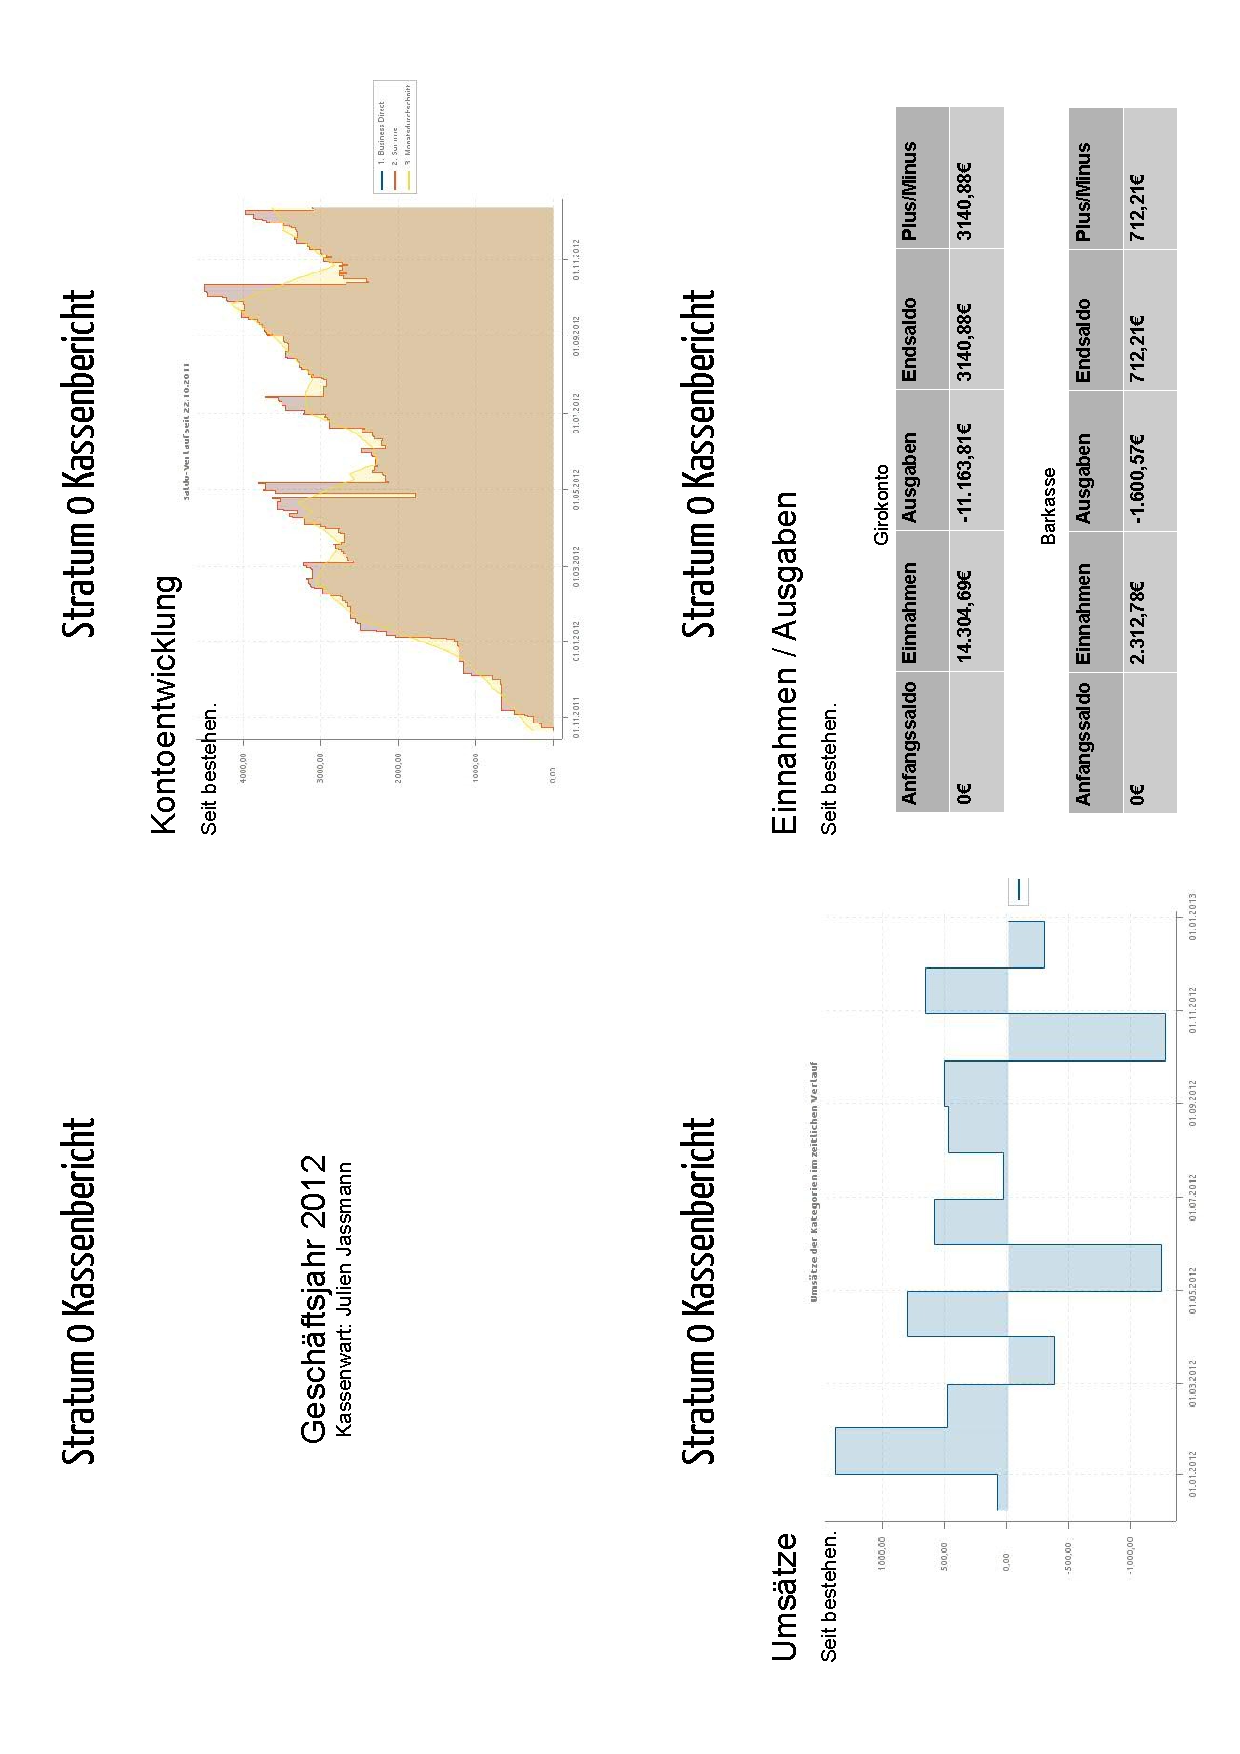
\includegraphics[width=\textwidth]{images/Kassenbericht_2012_1.pdf}
\newpage
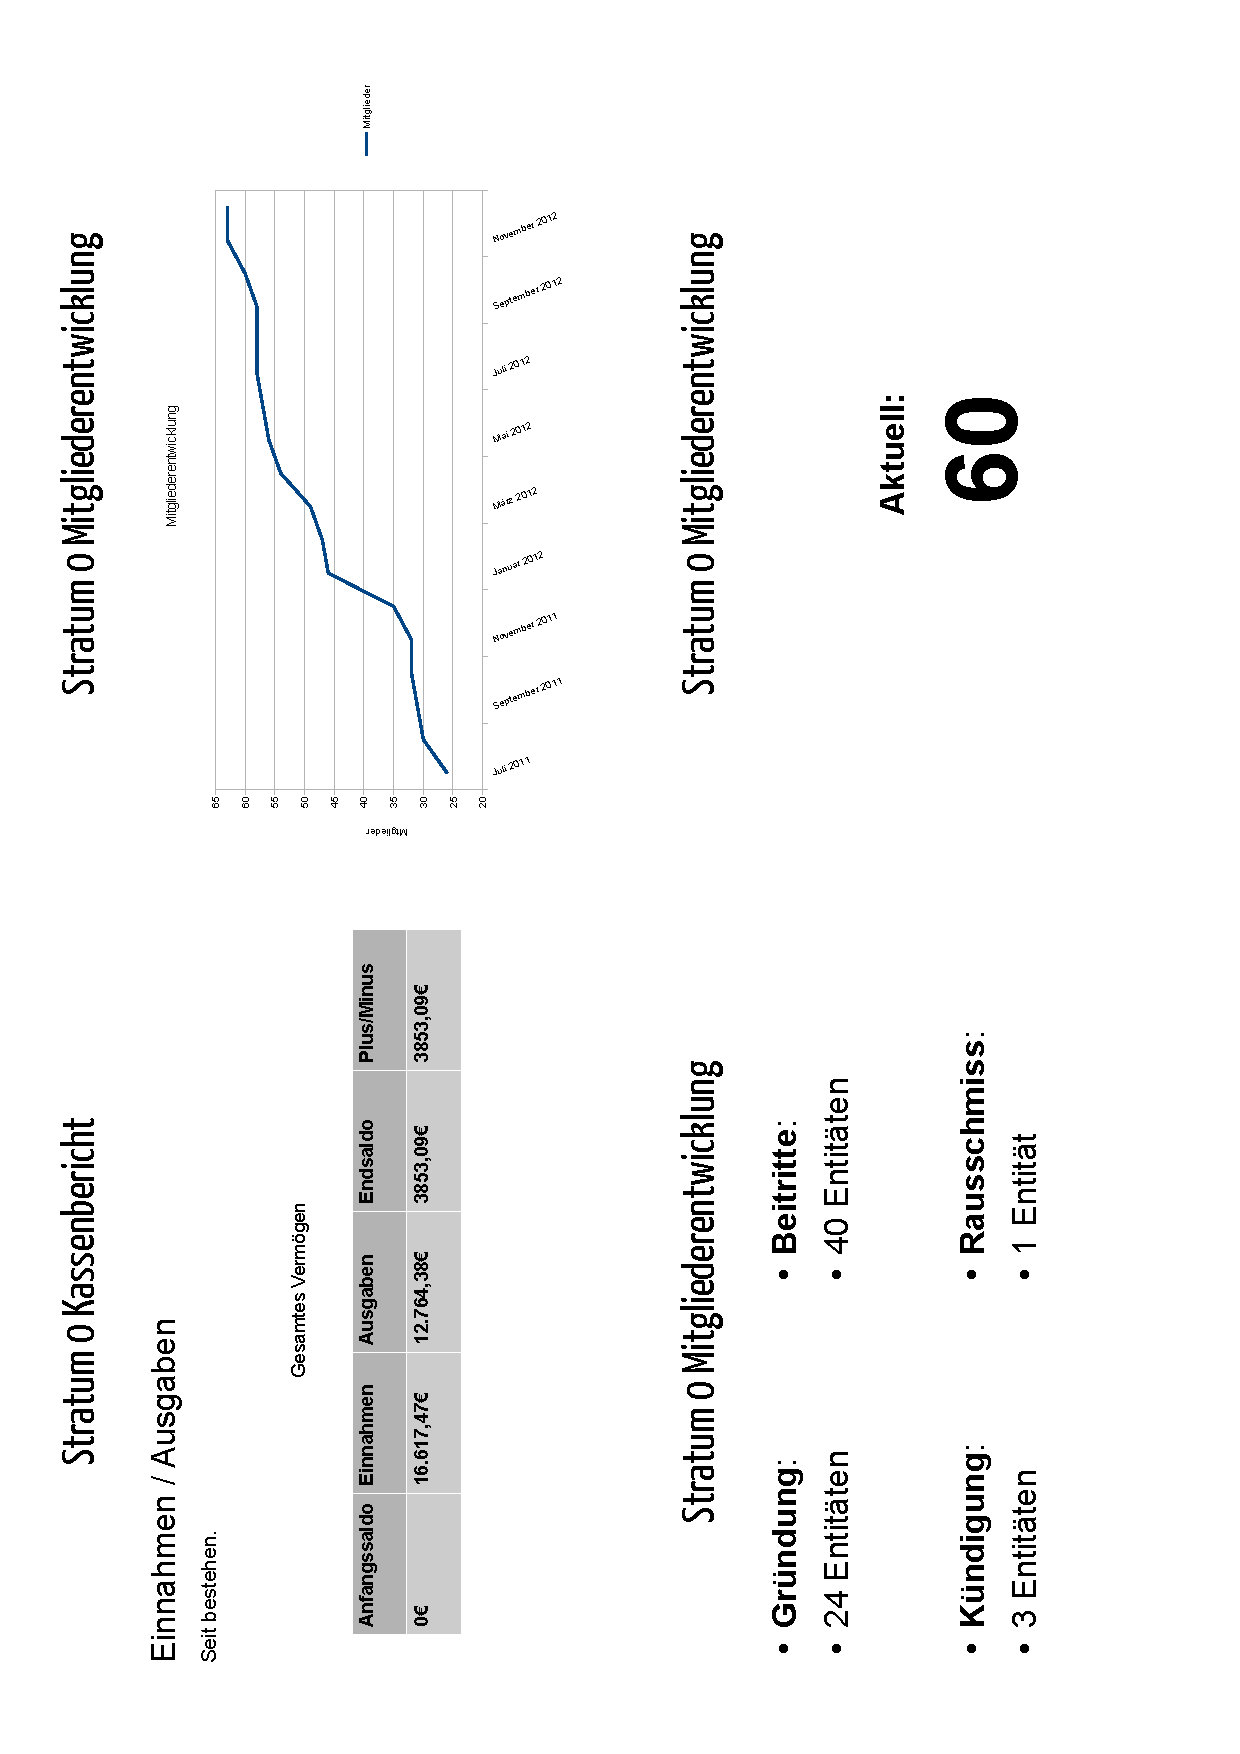
\includegraphics[width=\textwidth]{images/Kassenbericht_2012_2.pdf}

%%%%%%%%%%%%%%%%%%%%
%% Unterschriften %%
%%%%%%%%%%%%%%%%%%%%
\section{Unterschriften}
\vspace{0.7cm}
\noindent Protokollführer: \hrulefill\hfill\phantom{c}\par
\vspace{0.7cm}
\noindent Vorstandsvorsitzender: \hrulefill\hfill\phantom{c}\par
\vspace{0.7cm}
\noindent Stellv. Vorsitzender: \hrulefill\hfill\phantom{c}\par
\vspace{0.7cm}
\noindent Schatzmeister: \hrulefill\hfill\phantom{c}\par
\vspace{0.7cm}
\noindent Beisitzer: \hrulefill\hfill\phantom{c}\par
\vspace{0.7cm}
\noindent Beisitzer: \hrulefill\hfill\phantom{c}\par
\vspace{0.7cm}
\noindent Beisitzer: \hrulefill\hfill\phantom{c}\par

\end{document}
% vim: set tw=80 et sw=2 ts=2:
